\section{Quotienten von Ringen und Moduln}

Seien $M$ und $M'$ zwei $R$-Moduln und $N\subseteq M$ ein Untermodul.

\begin{definition}[Quotientenmodul]
	Für $x\in M$ schreiben wir
	\begin{align}
		x+N:=\{x+y\mid y\in N\}\notag
	\end{align}
	Der \begriff{Quotientenmodul} (oder Faktormodul) von $M$ modulo $N$ ist
	\begin{align}
		\qraum{M}{N}:=\{x+N\mid x\in M\}\notag
	\end{align}
	zusammen mit der Addition
	\begin{align}
		(x+N)+(y+N):=(x+y)+N\quad (x,y\in M)\notag
	\end{align}
	und der Skalarmultiplikation
	\begin{align}
		r\cdot (x+N) := rx+N\quad (x\in M,r\in R)\notag
	\end{align}
	Sei $\pi_N:M\to \qraum{M}{N}$ die Abbildung gegeben durch $x\mapsto x+N$.
\end{definition}

\begin{lemma}
	Addition und Skalarmultiplikation sind wohldefiniert und machen $\qraum{M}{N}$ zu einem $R$-Modul. Die Abbildung $\pi_N:M\to \qraum{M}{N}$ ist ein $R$-Epimorphismus mit Kern
	\begin{align}
		\Ker(\pi_N)=N\notag
	\end{align}
\end{lemma}
\begin{proof}
	\begin{itemize}
		\item wohldefiniert: wie in LAAG 1 III.7.5 %TODO: Verlinkung
		\item $\qraum{M}{N}$ ist $R$-Modul: wie in LAAG 1 III.7.7 %TODO: Verlinkung
	\end{itemize}
\end{proof}

\begin{remark}
	Durch $x\sim_N x' \iff x-x'\in N$ wird eine Äquivalenzrelation $\sim_N$ auf $M$ definiert, und $x+N$ ist eine $\sim_N$-Äquivalenzklasse $[x]_{\sim_N}=\{y\in M\mid x\sim_N y\}$.
\end{remark}

\begin{proposition}[Homomorphiesatz für Moduln]
	Sei $f\in\Hom_K(M,M')$ und $N\subseteq M$ ein Untermodul mit $N\subseteq \Ker(f)$. Dann gibt es genau ein $\overline{f}\in\Hom_K(\qraum{M}{N},M')$ mit $f=\overline{f}\circ \pi_N$.
	\begin{center}
		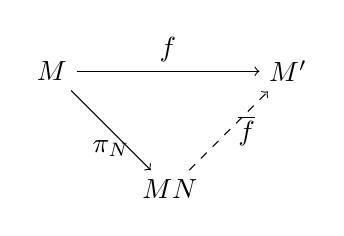
\begin{tikzpicture}
		\node (M) at (0,0) {$M$};
		\node (MS) at (3,0) {$M'$};
		\node (Q) at (1.5,-1.5) {\qraum{$M$}{$N$}};
		\draw[->, above] (M) to node {$f$} (MS);
		\draw[->, below] (M)  to node {$\pi_N$} (Q);
		\draw[->, right, dashed] (Q)  to node {$\overline{f}$} (MS);
		\end{tikzpicture}
	\end{center}
\end{proposition}
\begin{proof}
	Analog zu LAAG 1 III.7.9. Man zeigt, dass jedes $\overline{f}\in\Hom_K(\qraum{M}{N},M')$
	\begin{align}
		\overline{f}(x+N)=f(x)\quad (x\in M)\notag
	\end{align}
	erfüllen muss, und dass dies wiederum eine wohldefinierte Abbildung liefert. %TODO: Verlinkung
\end{proof}

\begin{lemma}
	Durch $U\mapsto \pi_N(U)$ wird eine Bijektion gegeben zwischen
	\begin{itemize}
		\item den Untermoduln von $M$, die $N$ enthalten
		\item den Untermoduln von $\qraum{M}{N}$.
	\end{itemize}
\end{lemma}
\begin{proof}
	Sei $\mathcal{U}$ die Menge der Untermoduln von $M$, die $N$ enthalten, $\overline{\mathcal{U}}$ die Menge der Untermoduln von $\qraum{M}{N}$.
	\begin{itemize}
		\item $U\in\mathcal{U}\Rightarrow \pi_N(U)\in\overline{\mathcal{U}}$: klar, da $\pi_N$ ein Homomorphismus ist
		\item $\overline{U}\in\overline{\mathcal{U}}\Rightarrow \pi_N^{-1}\in\mathcal{U}$: klar, da $\pi_N$ ein Homomorphismus ist und $N=\Ker(\pi_N)=\pi_N^{-1}(\{0\})\subseteq \pi_N^{-1}(\overline{U})$
		\item $\overline{U}\in\overline{\mathcal{U}}\Rightarrow\pi_N(\pi_N^{-1}(\overline{U}))=\overline{U}$: klar, da $\pi_N$ surjektiv
		\item $U\in\mathcal{U}\Rightarrow \pi_N^{-1}(\pi_N(U))=U$:
		\begin{align}
			\pi_N^{-1}(\pi_N(U)) &= \bigcup_{x\in U} \pi_N^{-1}(\pi_N(x)) \notag \\
			&= \bigcup_{x\in U} \pi_N^{-1}(x+N) \notag \\
			&= \bigcup_{x\in U}(x+N) \notag \\
			&= U+N=U\notag
		\end{align}
	\end{itemize}
\end{proof}